\section{Graph-Isomorphie und Color Refinement}
\label{sec/gi_cr}

\subsection{Graph-Isomorphie}
Zwei Graphen $G$ und $H$ sind isomorph, kurz $G\simeq H$, wenn es eine bijektive Abbildung $\phi$ der Knoten von $G$ auf $H$ gibt, sodass die Adjazenz aller Knoten erhalten bleibt. Es gilt also: $(u,v)\in E_G\Leftrightarrow (\phi (u),\phi (v))\in E_H$ für alle $u,v\in V_G$. Eine so definierte Abbildung $\phi$ wird \emph{Isomorphismus} genannt.

Es wurde gezeigt, dass das Graph-Isomorphie-Problem in $NP$ liegt, die $NP$-Vollständigkeit ist allerdings noch unklar. Es konnte außerdem noch kein Algorithmus gefunden werden, welcher das Problem in polynomieller Zeit löst, jedoch wird davon ausgegangen, dass es nicht $NP$-vollständig ist. Siehe \cite{Goldreich1991}.

\subsection{Color Refinement}
Der Color Refinement Algorithmus stellt eine Heuristik dar, mit der in polynomieller Zeit festgestellt werden kann, dass zwei Graphen nicht isomorph sind. Der Algorithmus geht wie folgt vor.
\begin{enumerate}
	\item Sämtliche Knoten des Graphen werden in der selben Farbe gefärbt.
	\item Die Knotenfärbungen werden verfeinert, indem überprüft wird, ob zwei Knoten gleicher Farbe unterschiedliche \glspl{nachbarschaft} mit Berücksichtigung der Farbe besitzen. Ist dies der Fall, werden die Knoten in unterschiedlichen Farben gefärbt und das Verfeinern wird fortgeführt.
	\item Ist die Bedingung für kein Knotenpaar mehr erfüllt, terminiert der Algorithmus.
	\item Sind die \glspl{multimenge} der Farben beider Graphen unterschiedlich, sind diese nicht isomorph.
\end{enumerate}

Es kann bei diesem Vorgehen vorkommen, dass zwei nicht isomorphe Graphen $G$ und $H$ nicht voneinander unterschieden werden können. Ein Beispiel hierfür wird in Abbildung \ref{fig:nicht_isomorphe_graphen} dargestellt. Zu erkennen ist, dass alle Knoten beider Graphen initial in einer Farbe gefärbt wurden, danach allerdings kein Verfeinerungsschritt mehr nötig ist, da die Nachbarschaften aller Knoten identisch gefärbt sind. Obwohl offensichtlich erkennbar ist, dass die beiden Graphen nicht isomorph sind, gelingt es dem Algorithmus also nicht diese zu unterscheiden. Auf Basis dieser Erkenntnisse wird die folgende Klasse von Graphen definiert.

\begin{Definition}
	Ein Graph $G$ wird \emph{CR-Graph} genannt, wenn der Color Refinement Algorithmus diesen von jedem beliebigen, nicht zu $G$ isomorphen Graphen $H$ unterscheiden kann. Die Arbeit, auf der diese Ausarbeitung beruht (\cite{Arvind2015}) nennt diese Kerneigenschaft von CR-Graphen \emph{amenable}
	\label{def:cr-graph1}
\end{Definition}

\begin{figure}[h]
	\centering
	\fbox{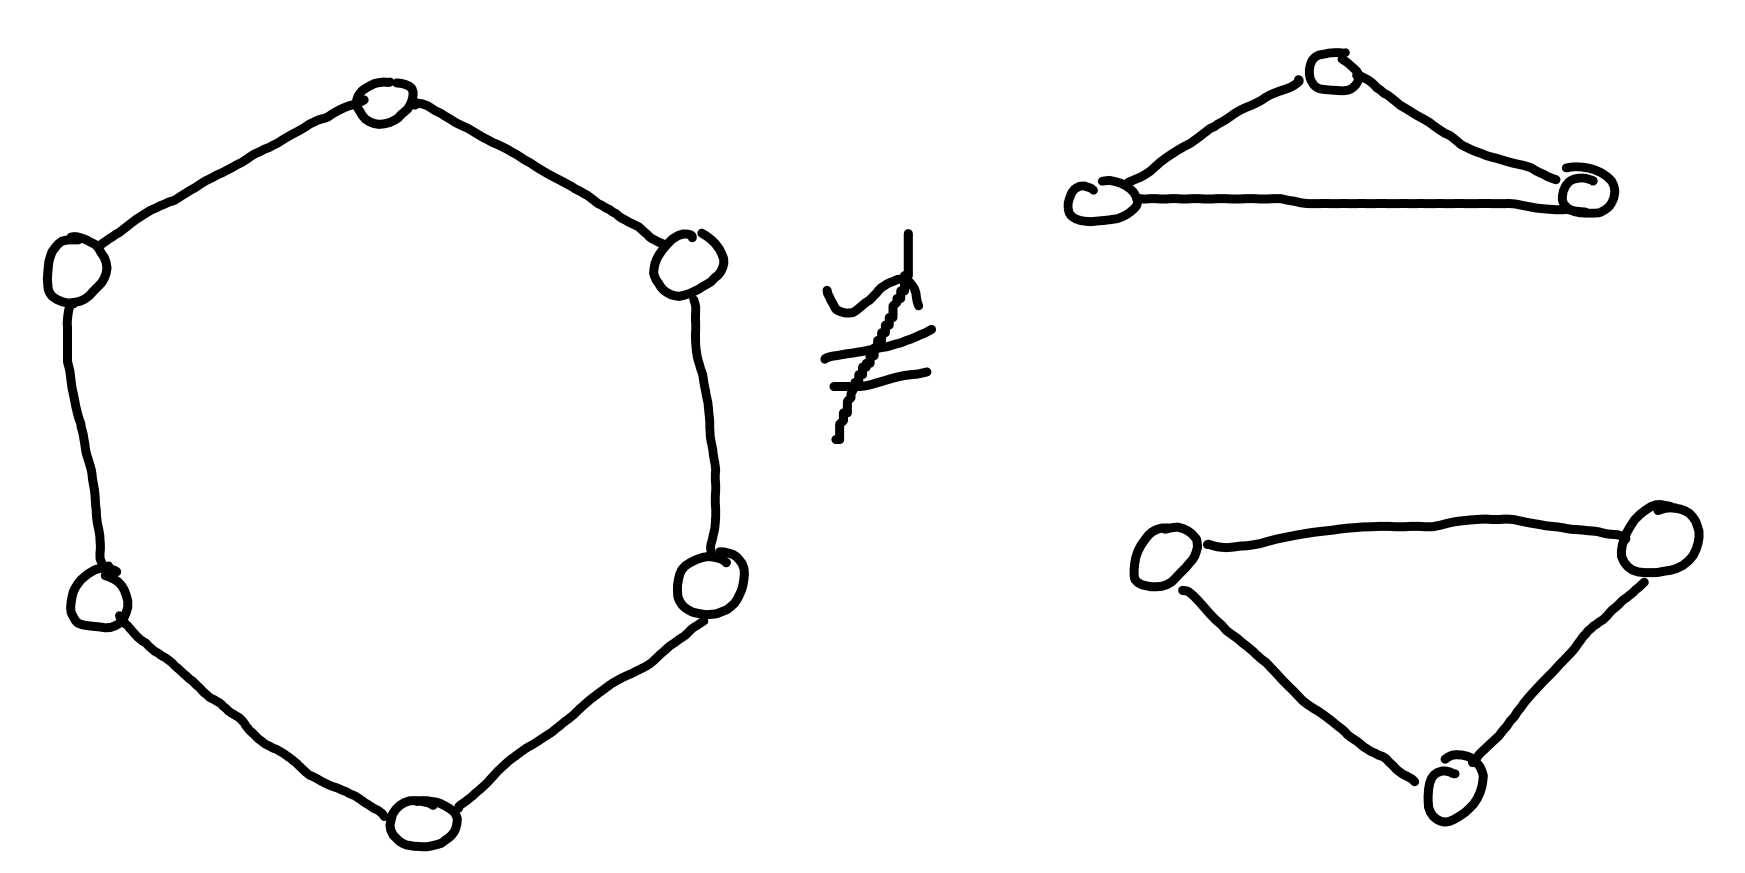
\includegraphics[width=0.75\textwidth]{./img/nicht_isomorphe_graphen.png}}
	\caption{Zwei nicht isomorphe Graphen, welche vom Color Refinement nicht unterschieden werden können}
	\label{fig:nicht_isomorphe_graphen}
\end{figure}

Neben dem klassischen Isomorphie-Test ist der Color Refinement Algorithmus auch für andere Anwendungsfelder geeignet. Als Beispiel ist hier die Verkleinerung von linearen Programmen durch Reduktion der Dimensionen der Gleichungssysteme und somit eine Erhöhung der Effizienz zu nennen. Siehe \cite{Grohe2014}. Weitere Anwendungsfelder finden sich in \cite{shervashidze2011weisfeiler} und \cite{kersting2014power}.

\subsection{Formale Definition von CR-Graphen}
Der Color Refinement Algorithmus berechnet iterativ eine Sequenz von Knotenfärbungen $C^i$ für einen Graphen $G$. Die initiale Färbung $C^i$ weist jedem Knoten die selbe Farbe zu. Nachfolgend wird in jeder Iteration nach folgender Regel eine neue Färbung gebildet.
\begin{equation}
C^{i+1}(u)=(C^i(u),\ldblbrace C^i(a):a\in N(u)\rdblbrace )
\label{eq:1}
\end{equation}
Die doppelten geschweiften Klammern $\ldblbrace \rdblbrace $ markieren hierbei eine \gls{multimenge}. Die Knoten von $G$ werden mithilfe einer Partitionierung $\mathcal{P}$ in die entsprechenden Farbklassen unterteilt, wodurch also zu jeder Färbung $C^i$ eine Partition $\mathcal{P}^i$ gehört.

Bei der Ausführung des Algorithmus wird irgendwann eine Partitionierung erreicht, die sich bei weiteren Verfeinerungsschritten nicht mehr verändert, da keine neue Färbung mehr generiert wird. Für diese gilt das Folgende.
\begin{Definition}
	Wenn sich eine Partitionierung bei weiteren Verfeinerungsschritten nicht mehr verändert, stellt dies die stabile Partitionierung $\mathcal{P}^s$ dar. Für sie gilt $\mathcal{P}^s=\mathcal{P}^i$ für alle $i\geq s$.
\end{Definition}
Die stabile Partitionierung ist bei jedem Graphen nach maximal $n-1$ Verfeinerungsschritten erreicht, da spätestens dann jeder Knoten eine unterschiedliche Farbe besitzt und somit keine weitere Verfeinerung mehr möglich ist.

Eine Partitionierung kann außerdem die Eigenschaft \emph{equitable} haben. Dafür müssen die im Folgenden definierten Eigenschaften erfüllt sein. Die Elemente der Partitionierung werden hier Zellen genannt.
\begin{Definition}
	Eine Partitionierung wird \emph{equitable} genannt, wenn die folgenden Eigenschaften erfüllt sind:
	\begin{enumerate}
		\item Jede Zelle $X\in \mathcal{P}$ ist einfarbig und enthält somit nur Knoten einer einzigen Farbe.
		\item Für jede Zelle $X\in \mathcal{P}$ ist der Graph $G[X]$ ein regulärer Graph.
		\item Für beliebige Zellen $X,Y\in \mathcal{P}$ ist der bipartite Graph $G[X,Y]$ ein biregulärer Graph.
	\end{enumerate}
\end{Definition}
Es ist somit leicht zu erkennen, dass die durch das Color Refinement erstellte stabile Partitionierung $\mathcal{P}^s$ equitable ist.

Eine weitere Eigenschaft der Graphfärbungen $C^i$ ist der Erhalt der Färbung über Isomorphismen hinweg.
\begin{Lemma}
	Für die Färbungen zweier isomorpher Graphen $G$ und $H$ und ihren Isomorphismus $\phi$ muss gelten: $C^i(u)=C^i(\phi (u))$ für alle $u\in V_G$.
\end{Lemma}
Aus dieser Aussage leitet sich die folgende Gleichung her.
\begin{equation}
\forall i\geq 0:{{C^i(u):u\in V_G}}=\ldblbrace C^i(v):v\in V_H\rdblbrace 
\label{eq:2}
\end{equation}
Das Color Refinement akzeptiert somit zwei Graphen $G$ und $H$ bei der Eingabe der \glslink{disjunkte_vereinigung}{disjunkten Vereinigung} $G+H$ genau dann, wenn die Gleichung (\ref{eq:2}) erfüllt ist.

Das Überprüfen dieser Bedingung ist in endlicher Zeit berechenbar. Für einen Zeugen $i$ dafür, dass die Gleichung nicht erfüllt ist, gilt $i<2n$, wobei $n$ die Anzahl der Knoten jedes Graphens ist. Dies beruht darauf, dass $\mathcal{P}^{2n-1}$ in jedem Fall die stabile Partitionierung von $G+H$ ist und weitere Verfeinerungsschritte keine neue Partitionierung erstellen würden. Es genügt sogar die Gleichung für $i=n$ zu verifizieren, da die Existenz einer Partitionierung $\mathcal{P}^{i+1}\neq \mathcal{P}^i$ bedeuten würde, dass es mehr als $n$ Partitionen, da in jedem Partitionierungsschritt mindestens eine Partition hinzukommt. Mehr als $n$ Partitionen sind ein Indikator dafür, dass die Graphen $G$ und $H$ nicht isomorph sind, da die $n$ Knoten jedes Graphen unmöglich in mehr als $n$ Partitionen unterteilt werden können und Gleichheit somit ausgeschlossen ist.

Aus den gewonnenen Erkenntnissen ergibt sich folgende Erweiterung zu Definition \ref{def:cr-graph1}.
\begin{Definition}
	Ein Graph $G$ wird \emph{CR-Graph} genannt, wenn für jeden beliebigen, nicht isomorphen Graphen $H$ die Gleichung (\ref{eq:2}) für $i=n$ nicht erfüllt ist.
\end{Definition}